\section{Evaluation}\label{eva}
This section describes our SW/HW co-design evaluation methodology. We evaluate our design using a Plant-on-Chip (PoC), which emulates the physical behavior of a linear system~\cite{VyaKum13A}. We provide post place\&route results including resource usage and maximum clock frequency. We then compare our work with other related works.
\subsection{Mass-spring System}
The system we use to test our controller is a mass-spring model, which is considered as a benchmark in \cite{6927473}, \cite{Jerez:2011:FIS:1950413.1950454} and many recent works use it to validate their hardware controller. The physical system is illustrated in Fig.~\ref{fig_ms}. The objective is moving masses to desired positions by applying a force to each mass. The state vector consists of the position ($P$) and speed ($\dot P$) of each mass\footnote{$P$ is the position relative to the initial position}. The state space model size increases quadratically as the number of masses increases. We constrain the position of each mass within 0.5m to avoid collision between adjacent masses. Each mass is 1Kg, and the spring constant is 1N/m. The input force ($U$) is limited to $\pm 0.5N$ and the change of input force between each sample period (i.e. rate of change, $\Delta U$) is 0.1N, as in \cite{jerez2014embedded}. The sample period is 0.1s. The prediction horizon ($H_p$) and input horizon ($H_u$) are both 12. The cost constant for position $P$, input force $U$ and input-rate $\Delta U$ are 80, 1 and 0 (we are not trying to minimize $\Delta U$ during the control process) respectively.

\begin{figure}[t]
\centering
\captionsetup{justification=centering}
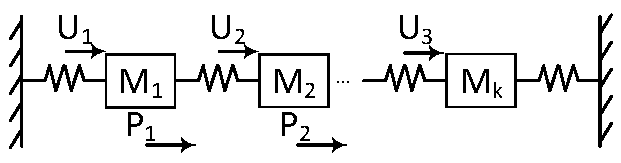
\includegraphics[scale=.48]{../figure/massspring.pdf}
\DeclareGraphicsExtensions.
\caption{Mass-spring System\label{fig_ms}}
\end{figure}

\subsection{Plant on Chip Emulation}
We conducted our experiments on a Zynq-7020 device. A Plant-on-Chip (PoC) was deployed onto the FPGA's Programable Logic (PL) fabric to emulate the mass-spring system shown in Fig.~\ref{fig_ms}. The PoC executes state space Equations~\ref{eq:xk} and~\ref{eq:yk} with input $u_k$ received from a hardware or software-based controller. The state of the PoC and control commands are logged out of band, using a UART interface, which is convenient for plotting the controller behavior at runtime.\par
The MPC controller requires the CPU to configure the co-processor BRAM content with the matrix $M_{11}$. When running the MPC hardware controller at 100 MHz, it computes $u_k$ in 347.8$\mu s$ using a $D_p$=3 MVM tree and executes 20 fixed converge iterations.\par
The hardware control graph is shown in Fig.~\ref{fig_mp}. The red dashed line is the software configured trajectory, and the blue line is the actual mass position. The first 100 points of the trajectory are stored in the trajectory FIFO during configuration, which reflects 0s$-$10s of red trajectory line. The remainder of the trajectory is configured during runtime. The input force and the input force rate of change are shown in Fig.~\ref{fig_mu}. From the graph, we can see that the control signal and control signal rate of change respect their bounding constraints of $\pm$0.5N and $\pm$0.1N per time step respectively.

\begin{figure}[t]
\centering
\captionsetup{justification=centering}
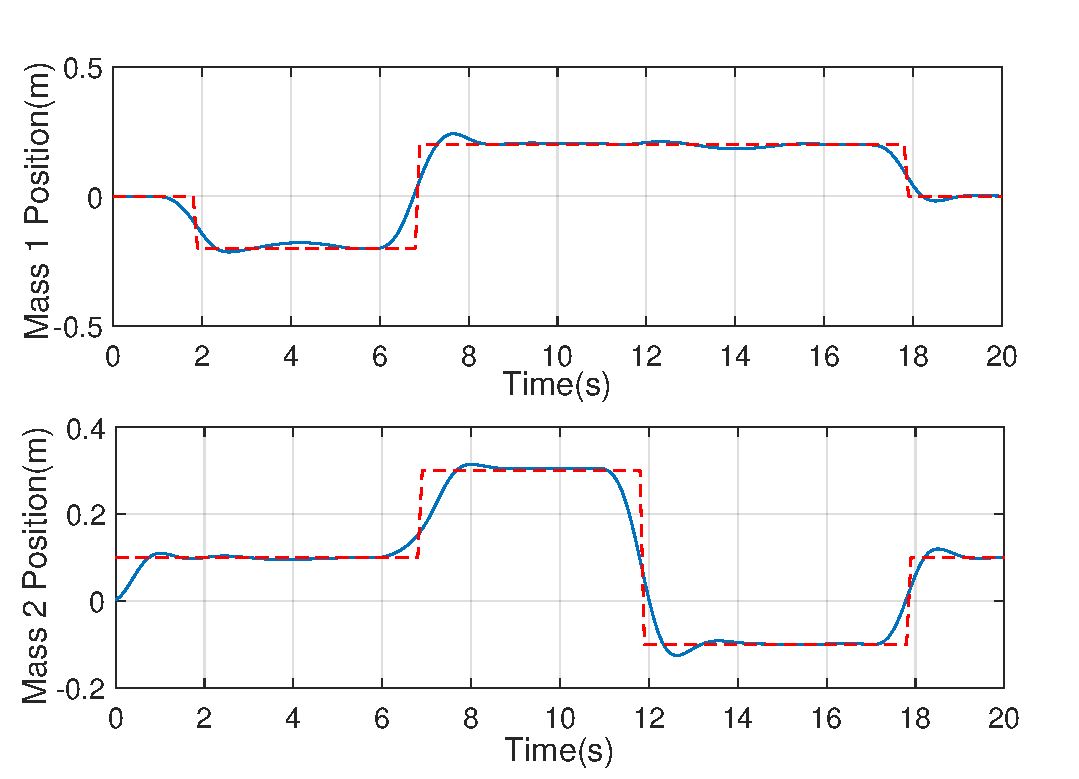
\includegraphics[scale=.45]{../figure/MP.pdf}
\DeclareGraphicsExtensions.
\caption{Mass Position Change with respect to Planned Trajectory. Red dashed line is the planned trajectory, and the blue line is the actual trajectory.\label{fig_mp}}
\end{figure}

\begin{figure}[t]
\centering
\captionsetup{justification=centering}
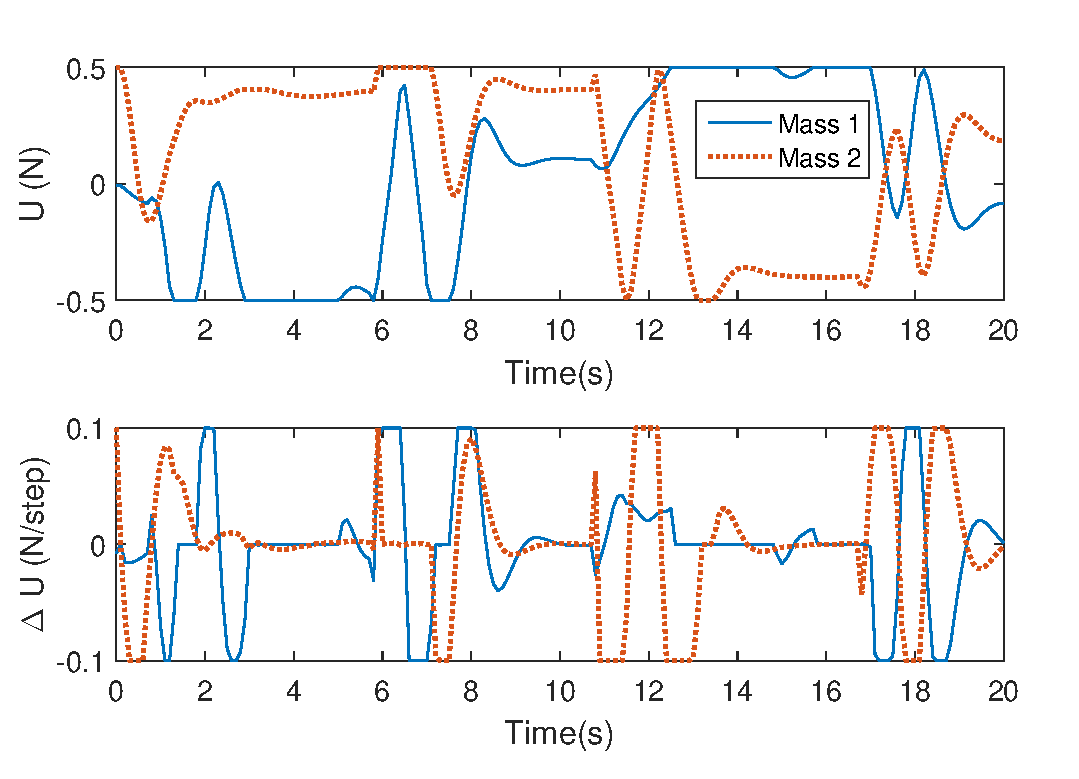
\includegraphics[scale=.45]{../figure/MU.pdf}
\DeclareGraphicsExtensions.
\caption{Control Signal $U$ and $\Delta U$. Blue line is the input force and the force rate of change for $M_1$, red dashed line is for $M_2$.\label{fig_mu}}
\end{figure}

\subsection{SW/HW Co-design}
The on-chip ARM processor transfers a pre-generated $M_{11}$ matrix into the reconfigurable fabric's BRAMs through the AXI bus. Additionally, the on-chip ARM processor can access memory-mapped registers resident in the reconfigurable fabric to indicate when the MPC hardware engine should start and stop, and for updating the desired trajectory at runtime.
The system block design is shown in Fig.~\ref{fig_copro}. The design steps are:
\begin{enumerate}
\item According to system requirements, generate the bitstream in Vivado, and $M_{11}$ matrix in Matlab.
\item Store $M_{11}$ to BRAM via AXI bus using ARM software.
\item ARM software configures trajectory and box constraints.
\item Send start signal to the PoC, and collect data through UART to external computer and plot graph.
\end{enumerate}\par
As we can see from the design steps, a control engineer can easily handle each step. In addition, when we apply the hardware control to another system with different parameters and size, the design can be easily adjusted.
% For the control interface design example between FPGA and physical plant, refer to\cite{telba2015dc}.

\begin{figure}[t]
\centering
\captionsetup{justification=centering}
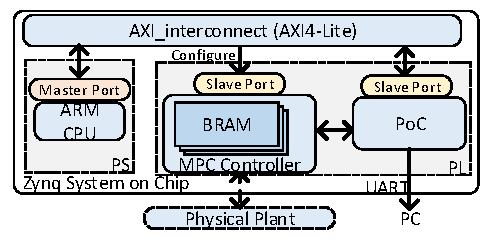
\includegraphics[scale=.84]{../figure/copro.pdf}
\DeclareGraphicsExtensions.
\caption{Top Level System Overview\label{fig_copro}}
\end{figure}


\begin{figure}[t]
\centering
\captionsetup{justification=centering}
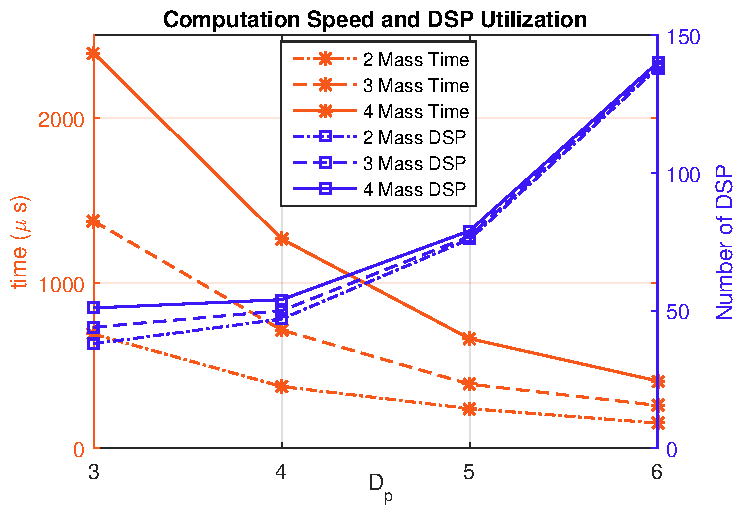
\includegraphics[scale=.65]{../figure/dsp.pdf}
\DeclareGraphicsExtensions.
\caption{Computation time of 40 converge iteration loops and DSP usage for different system configurations from simulation. Computation time is marked by $\ast$, number of DSPs is marked by $\Box$. Hardware speed is 100MHz.\label{fig_ct}}
\end{figure}

\subsection{Computation Speed Versus Hardware Resources}
The relationship between DSP usage, $D_p$, and system size is shown in Fig.\cref{fig_ct}. As $D_p$ increases, the size of the reduce circuit will decrease thus reducing computation time. The DSP resources used is modifiable. The more DSPs we use, the faster computation speed we achieve. Consider a situation where an FPGA has few DSP resources available, our proposed architecture can still execute the controller by decreasing the MVM depth, at the cost of increased computing time.\par

\subsection{Resource Utilization and Timing Summary}
Table~\ref{tab_hrs} shows the resource utilization of the ADMM architecture. Each floating-point multiplier and adder use one DSP48E. We used the maximum number of pipeline stages supported by the Xilinx floating point adder(11) and multiplier(8) IP cores. Each memory attached to the MVM multiplier tree is composed of 2 36Kb BRAMs. BRAMs are also used for FIFOs in the MVM tree and Bottom level. The Zynq-7020 can hold an MVM tree having a depth up to 6. Generally, the clock frequency can easily reach 100MHz. 
\begin{table}[!ht]
\centering
\captionsetup{justification=centering}
\caption{Zynq-7020 Hardware Resource Usage}\label{tab_hrs}
\begin{tabular}{ >{\centering\arraybackslash} m{0.6cm} |>{\centering\arraybackslash} m{0.9cm}|>{\centering\arraybackslash} m{0.9cm}|>{\centering\arraybackslash} m{0.9cm}|>{\centering\arraybackslash} m{0.85cm}|>{\centering\arraybackslash} m{1cm} }

\hline
\multicolumn{1}{c|}{MVM}&\multicolumn{1}{c|}{Flip-Flops}&\multicolumn{1}{c|}{LUTs}&\multicolumn{1}{c|}{18Kb }&\multicolumn{1}{c|}{DSP48E}&\multicolumn{1}{c}{Maximum }\\

Size $D_p$ &(106400 total)&(53200 total)&BRAM (280 total)&(220 total)&Frequency \\ 
 
\hline

3&18147&12746&55&38&151.149MHz\\
\hline 
4& 21058 & 15103&87&47&144.885MHz\\
\hline 
5& 32425 & 23391 &151&76&143.699MHz\\
\hline 
6& 57167 & 41273&279&138&133.298MHz\\
\hline

\end{tabular}
\end{table}

We also tested the resource scaling on a Zynq Ultrascale. It can reach 340MHz when deploying a $D_p=8$ MVM tree.

%\subsection{Single Precision Floating Point Error}
%We compare the single precision floating point with double precision floating point by running the mass spring system with ADMM iteration ranging from 10 to 40. The error is shown in Table.~\ref{tab_pe}. We also show the error between 20 bit fraction fixed point and double precison floating point.
%
%\begin{table}[!ht]
%\centering
%\captionsetup{justification=centering}
%\caption{Percentage of Error using FLoating Point and Fixed Point(20 bit fraction per iteration. $I$ means the total number of iterations) in each iteration.}\label{tab_pe}
%\begin{tabular}{ >{\centering\arraybackslash} m{0.6cm} |>{\centering\arraybackslash} m{0.6cm}|>{\centering\arraybackslash} m{0.6cm}|>{\centering\arraybackslash} m{0.6cm}|>{\centering\arraybackslash} m{0.6cm}|>{\centering\arraybackslash} m{0.6cm}| >{\centering\arraybackslash} m{0.6cm}| >{\centering\arraybackslash} m{0.6cm} }
%
%\hline
%\multicolumn{1}{c|}{Type $\backslash$ I}&\multicolumn{1}{c|}{10}&\multicolumn{1}{c|}{15}&\multicolumn{1}{c|}{20 }&\multicolumn{1}{c|}{25}&\multicolumn{1}{c|}{30}&\multicolumn{1}{c|}{35}&\multicolumn{1}{c}{40}\\
%\hline
%SP&7.3&1.8&2.4&1.7&1.3&0.75&0.12\\
%Floating&e-6&e-6&e-6&e-6&e-6&e-6&e-6\\
%\hline 
%Fixed& 0.58 & 0.49 & 0.42 & 0.37 & 0.32 & 0.28 & 0.25\\
%\hline
%\end{tabular}
%\end{table}
%
%We find that floating point error is much smaller than 20 fractional fixed point. Thus we run our experiment only use 20 iterations.

\subsection{Comparision with other Works}
Table~\ref{tab_cmp} provides a comparative summary of our work with two other FPGA accelerated MPC works and a software implementation. For the hardware work, one is IPM based \cite{6927473}, and another is ADMM based \cite{jerez2014embedded}, like ours. Starting with the IPM based work, it can be seen when compared against the ADMM-based approaches using about half the number of multipliers (\textasciitilde{200}) for about the same number of decision variables (\textasciitilde{200}) our approach is about 50x faster (2,650us vs. 46.1us) than the IPM implementation and the other ADMM work \cite{jerez2014embedded} is about 100x faster (2,650us vs. 23.4us). As explained in Section~\ref{rw}, this is due to the ADMM algorithm requiring less computation per convergence iteration. The software implementation, \cite{6422363}, is ADMM based, and is run on a 3.4GHz Xeon processor. We estimate for 262 variables that this SW solution would take 850 $\mu s$ if the average number of iteration maintains in 35.1.\par
 \begin{table*}[!ht]
\small
\centering
\captionsetup{justification=centering}
\caption[Caption for LOF]{Hardware Computation Time per Iteration between Related Work.\label{tab_cmp}\protect\footnotemark}
%\caption{Hardware Computation Time per Iteration between Related Work.\label{tab_cmp}}

\begin{tabular}{|*{9}{c|}}\hline

&\makebox[2.2em]{Method}&\makebox[4em]{Data Format}&\makebox[4em]{Chip Series}&\makebox[2.5em]{$f_{clk}$}&\makebox[4em]{\#Multipliers}&\makebox[2.5em]{Iteration}&\makebox[3em]{\#Opt Var}&\makebox[6em]{Running Time}\\
\hline
\hline

\multirow{5}{*}{This Paper} &\multirow{5}{*}{ADMM}&\multirow{5}{*}{floating-point}&\multirow{3}{*}{Zynq-7020}&\multirow{3}{*}{130MHz}&\multirow{2}{*}{72 ($D_p$=6, K=1)}&\multirow{5}{*}{40}&\multirow{1}{*}{204}&\multirow{1}{*}{314.2 $\mu s$}\\
\hhline{~~~~~~~--}
&&&\multirow{0}{*}{}&&&&350*&{717.2 $\mu s$}\\
\hhline{~~~~~-~--} 
&&&\multirow{1}{*}{}&&80 ($D_p$=5, K=2)&&\multirow{3}{*}{204}&{291.4 $\mu s$}\\
\hhline{~~~---~~-}
&&&\multirow{1}{*}ZU9EG&\multirow{2}{*}{340MHz}&264 ($D_p$=8, K=1)&&&{46.1 $\mu s$}\\
\hhline{~~~~~-~~-}
&&&\multirow{1}{*}(Zynq UltraScale+)&&792 ($D_p$=8, K=3)&&&{30.1 $\mu s$}\\ 
\hline
\hline

\multirow{2}{*}{HW\cite{jerez2014embedded}} &\multirow{2}{*}{ADMM}&\multirow{2}{*}{fixed-point}&Virtex-6 (LX75)&\multirow{2}{*}{400MHz}&\multirow{1}{*}{216 (K=1)}&\multirow{2}{*}{40}&\multirow{2}{*}{216}&\multirow{1}{*}{23.4$\mu s$}\\ 
\hhline{*4~|*1~|*4~}
%&&&LX75&& &&&\\
\hhline{*3~|-|~|-|*2~|-}
\multirow{1}{*}{} &\multirow{1}{*}{}&\multirow{1}{*}{}&Virtex-6 (SX475)&\multirow{0}{*}{}&\multirow{1}{*}{1512 (K=7)}&\multirow{1}{*}{}&\multirow{1}{*}{}&\multirow{1}{*}{4.90$\mu s$}\\ 
\hhline{*4~|*1~|*4~}
%&&&SX475&& &&&\\
\hline
\hline

\multirow{1}{*}{HW\cite{6927473}} &\multirow{1}{*}{IPM}&\multirow{1}{*}{floating-point}&Virtex-7 (XC7VX485T)&\multirow{1}{*}{200MHz}&\multirow{1}{*}{448}&\multirow{1}{*}{10}&\multirow{1}{*}{240}&\multirow{1}{*}{2,650 $\mu s$}\\ 
\hhline{*9~}
%&&&(XC7VX485T)&&&&&\\
\hline
\hline

\multirow{1}{*}{SW\cite{6422363}} &\multirow{1}{*}{ADMM}&\multirow{1}{*}{floating-point}& Quad-core Intel
Xeon&\multirow{1}{*}{3.4GHz}&\multirow{1}{*}{n/a}&\multirow{1}{*}{35.1}&\multirow{1}{*}{525}&\multirow{1}{*}{3,400 $\mu s$}\\ 
\hhline{*9~}

\hline
\end{tabular}
\end{table*}

When comparing our approach with the ADMM based approach of \cite{jerez2014embedded}, for about 200 multipliers and 200 decision variables, it can be seen that our approach is about two times slower (i.e. 46.1 us vs. 23.4 us). The primary reason for this is that in \cite{jerez2014embedded} fixed point arithmetic is used, while our implementation uses 32-bit floating point arithmetic. The main way in which this impacts performance is that the floating point adders required 11 pipelining stages to maximize clock frequency, while fixed point addition can be done at a high clock rate in one clock cycle. For the size of matrices being operated on (limited by on-chip memory), the number of adder pipeline cycles to fill the processing pipeline (\textasciitilde{88} for an MVM tree of depth 8) is nearly half the number of matrix rows (\textasciitilde{200}) read into the MVM tree. This accounts for a vast majority of the two times difference in performance. However, for this cost in performance, we gain the convince of software and control algorithm developers not having to deal with the complexities of working with custom fixed-point number formats, easing the process of deploying a designed controller into our MPC accelerator. For physical systems requiring sub-millisecond controller updates rates, this is a good tradeoff, however for controllers requiring 10’s of microsecond updates rates using a fixed-point approach is more appropriate with today’s FPGA capabilities. The important question to answer is for your application is the convenience of using floating point worth the performance tradeoff.
 
The Reduce circuitry implemented in our architecture naturally allows our design to scale to large numbers of decision variables using a nearly arbitrarily small number of multipliers at the cost of speed, as is illustrated in the 350* entry of Table~\ref{tab_cmp}, while \cite{jerez2014embedded} does not have such a mechanism for scaling the number of decision variables above the number of multipliers in the system. This gives our MPC engine the flexibility to be deployed into System-on-Chip FPGA applications that may not have many multipliers to allocate to an MPC computation engine. Two ADMM tuning features implemented in our ADMM architecture that is not implemented by \cite{jerez2014embedded} is a relaxation parameter ($\alpha$) and a dual update step length ($\rho$), which can be used to tune the convergence rate of ADMM for a given system.

A final point of comparison is that this work tightly integrates an on-chip ARM processor with the MPC compute engine. This provides Controls or Software engineers a convenient software mechanism for configuring the controller for arbitrary systems, updating the desired trajectory of the system at runtime, and tuning the ADMM $\alpha$ and $\rho$ parameters.


\footnotetext{K indicates the number of times the core MPC engine with $D_p$ MVM tree is duplicated to process Matrix rows in parallel}

